\documentclass[10pt]{standalone}
\usepackage[sc]{mathpazo}
\usepackage{commands}

\begin{document}
    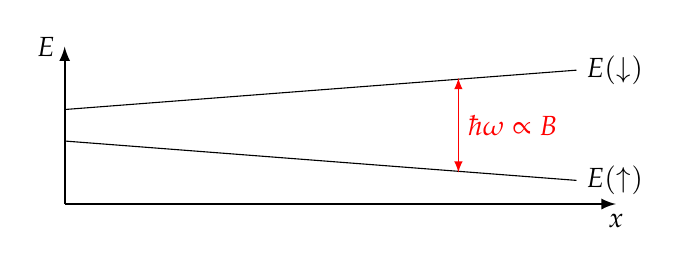
\begin{tikzpicture}
        \draw[-latex, thick] (0, 0) -- (0, 2);
        \draw[-latex, thick] (0, 0) -- (7, 0);
        \node[below] at (7, 0) {$x$};
        \node[left] at (0, 2) {$E$};
        \draw[] (0, 0.8) -- (6.5, 0.3);
        \node[right] at (6.5, 0.3) {$E(\uparrow)$};
        \draw[] (0, 1.2) -- (6.5, 1.7);
        \node[right] at (6.5, 1.7) {$E(\downarrow)$};
        \draw[latex-latex, red] (5, 0.4) -- (5, 1.6);
        \node[right, red] at (5, 1) {$\hbar\omega \propto B$};
    \end{tikzpicture}
\end{document}